% Options for packages loaded elsewhere
\PassOptionsToPackage{unicode}{hyperref}
\PassOptionsToPackage{hyphens}{url}
%
\documentclass[
  ignorenonframetext,
]{beamer}
\usepackage{pgfpages}
\setbeamertemplate{caption}[numbered]
\setbeamertemplate{caption label separator}{: }
\setbeamercolor{caption name}{fg=normal text.fg}
\beamertemplatenavigationsymbolsempty
% Prevent slide breaks in the middle of a paragraph
\widowpenalties 1 10000
\raggedbottom
\setbeamertemplate{part page}{
  \centering
  \begin{beamercolorbox}[sep=16pt,center]{part title}
    \usebeamerfont{part title}\insertpart\par
  \end{beamercolorbox}
}
\setbeamertemplate{section page}{
  \centering
  \begin{beamercolorbox}[sep=12pt,center]{part title}
    \usebeamerfont{section title}\insertsection\par
  \end{beamercolorbox}
}
\setbeamertemplate{subsection page}{
  \centering
  \begin{beamercolorbox}[sep=8pt,center]{part title}
    \usebeamerfont{subsection title}\insertsubsection\par
  \end{beamercolorbox}
}
\AtBeginPart{
  \frame{\partpage}
}
\AtBeginSection{
  \ifbibliography
  \else
    \frame{\sectionpage}
  \fi
}
\AtBeginSubsection{
  \frame{\subsectionpage}
}
\usepackage{amsmath,amssymb}
\usepackage{lmodern}
\usepackage{iftex}
\ifPDFTeX
  \usepackage[T1]{fontenc}
  \usepackage[utf8]{inputenc}
  \usepackage{textcomp} % provide euro and other symbols
\else % if luatex or xetex
  \usepackage{unicode-math}
  \defaultfontfeatures{Scale=MatchLowercase}
  \defaultfontfeatures[\rmfamily]{Ligatures=TeX,Scale=1}
\fi
% Use upquote if available, for straight quotes in verbatim environments
\IfFileExists{upquote.sty}{\usepackage{upquote}}{}
\IfFileExists{microtype.sty}{% use microtype if available
  \usepackage[]{microtype}
  \UseMicrotypeSet[protrusion]{basicmath} % disable protrusion for tt fonts
}{}
\makeatletter
\@ifundefined{KOMAClassName}{% if non-KOMA class
  \IfFileExists{parskip.sty}{%
    \usepackage{parskip}
  }{% else
    \setlength{\parindent}{0pt}
    \setlength{\parskip}{6pt plus 2pt minus 1pt}}
}{% if KOMA class
  \KOMAoptions{parskip=half}}
\makeatother
\usepackage{xcolor}
\newif\ifbibliography
\usepackage{color}
\usepackage{fancyvrb}
\newcommand{\VerbBar}{|}
\newcommand{\VERB}{\Verb[commandchars=\\\{\}]}
\DefineVerbatimEnvironment{Highlighting}{Verbatim}{commandchars=\\\{\}}
% Add ',fontsize=\small' for more characters per line
\usepackage{framed}
\definecolor{shadecolor}{RGB}{248,248,248}
\newenvironment{Shaded}{\begin{snugshade}}{\end{snugshade}}
\newcommand{\AlertTok}[1]{\textcolor[rgb]{0.94,0.16,0.16}{#1}}
\newcommand{\AnnotationTok}[1]{\textcolor[rgb]{0.56,0.35,0.01}{\textbf{\textit{#1}}}}
\newcommand{\AttributeTok}[1]{\textcolor[rgb]{0.77,0.63,0.00}{#1}}
\newcommand{\BaseNTok}[1]{\textcolor[rgb]{0.00,0.00,0.81}{#1}}
\newcommand{\BuiltInTok}[1]{#1}
\newcommand{\CharTok}[1]{\textcolor[rgb]{0.31,0.60,0.02}{#1}}
\newcommand{\CommentTok}[1]{\textcolor[rgb]{0.56,0.35,0.01}{\textit{#1}}}
\newcommand{\CommentVarTok}[1]{\textcolor[rgb]{0.56,0.35,0.01}{\textbf{\textit{#1}}}}
\newcommand{\ConstantTok}[1]{\textcolor[rgb]{0.00,0.00,0.00}{#1}}
\newcommand{\ControlFlowTok}[1]{\textcolor[rgb]{0.13,0.29,0.53}{\textbf{#1}}}
\newcommand{\DataTypeTok}[1]{\textcolor[rgb]{0.13,0.29,0.53}{#1}}
\newcommand{\DecValTok}[1]{\textcolor[rgb]{0.00,0.00,0.81}{#1}}
\newcommand{\DocumentationTok}[1]{\textcolor[rgb]{0.56,0.35,0.01}{\textbf{\textit{#1}}}}
\newcommand{\ErrorTok}[1]{\textcolor[rgb]{0.64,0.00,0.00}{\textbf{#1}}}
\newcommand{\ExtensionTok}[1]{#1}
\newcommand{\FloatTok}[1]{\textcolor[rgb]{0.00,0.00,0.81}{#1}}
\newcommand{\FunctionTok}[1]{\textcolor[rgb]{0.00,0.00,0.00}{#1}}
\newcommand{\ImportTok}[1]{#1}
\newcommand{\InformationTok}[1]{\textcolor[rgb]{0.56,0.35,0.01}{\textbf{\textit{#1}}}}
\newcommand{\KeywordTok}[1]{\textcolor[rgb]{0.13,0.29,0.53}{\textbf{#1}}}
\newcommand{\NormalTok}[1]{#1}
\newcommand{\OperatorTok}[1]{\textcolor[rgb]{0.81,0.36,0.00}{\textbf{#1}}}
\newcommand{\OtherTok}[1]{\textcolor[rgb]{0.56,0.35,0.01}{#1}}
\newcommand{\PreprocessorTok}[1]{\textcolor[rgb]{0.56,0.35,0.01}{\textit{#1}}}
\newcommand{\RegionMarkerTok}[1]{#1}
\newcommand{\SpecialCharTok}[1]{\textcolor[rgb]{0.00,0.00,0.00}{#1}}
\newcommand{\SpecialStringTok}[1]{\textcolor[rgb]{0.31,0.60,0.02}{#1}}
\newcommand{\StringTok}[1]{\textcolor[rgb]{0.31,0.60,0.02}{#1}}
\newcommand{\VariableTok}[1]{\textcolor[rgb]{0.00,0.00,0.00}{#1}}
\newcommand{\VerbatimStringTok}[1]{\textcolor[rgb]{0.31,0.60,0.02}{#1}}
\newcommand{\WarningTok}[1]{\textcolor[rgb]{0.56,0.35,0.01}{\textbf{\textit{#1}}}}
\usepackage{longtable,booktabs,array}
\usepackage{calc} % for calculating minipage widths
\usepackage{caption}
% Make caption package work with longtable
\makeatletter
\def\fnum@table{\tablename~\thetable}
\makeatother
\usepackage{graphicx}
\makeatletter
\def\maxwidth{\ifdim\Gin@nat@width>\linewidth\linewidth\else\Gin@nat@width\fi}
\def\maxheight{\ifdim\Gin@nat@height>\textheight\textheight\else\Gin@nat@height\fi}
\makeatother
% Scale images if necessary, so that they will not overflow the page
% margins by default, and it is still possible to overwrite the defaults
% using explicit options in \includegraphics[width, height, ...]{}
\setkeys{Gin}{width=\maxwidth,height=\maxheight,keepaspectratio}
% Set default figure placement to htbp
\makeatletter
\def\fps@figure{htbp}
\makeatother
\setlength{\emergencystretch}{3em} % prevent overfull lines
\providecommand{\tightlist}{%
  \setlength{\itemsep}{0pt}\setlength{\parskip}{0pt}}
\setcounter{secnumdepth}{-\maxdimen} % remove section numbering
\ifLuaTeX
  \usepackage{selnolig}  % disable illegal ligatures
\fi
\IfFileExists{bookmark.sty}{\usepackage{bookmark}}{\usepackage{hyperref}}
\IfFileExists{xurl.sty}{\usepackage{xurl}}{} % add URL line breaks if available
\urlstyle{same} % disable monospaced font for URLs
\hypersetup{
  pdftitle={Chapter 1: Interactive Notebook for Instructors},
  pdfauthor={Ram Gopal, Dan Philps, and Tillman Weyde},
  hidelinks,
  pdfcreator={LaTeX via pandoc}}

\title{Chapter 1: Interactive Notebook for Instructors}
\author{Ram Gopal, Dan Philps, and Tillman Weyde}
\date{Summer 2022}

\begin{document}
\frame{\titlepage}

\begin{frame}[fragile]{Simple Computations}
\protect\hypertarget{simple-computations}{}
Create a new script file. Let us begin with simple computations in R
using \texttt{*},\texttt{/},\texttt{sqrt()},\texttt{exp()}, and
\texttt{log()} operators and functions.

\begin{Shaded}
\begin{Highlighting}[]
\DecValTok{25}\SpecialCharTok{*}\DecValTok{77}  
\DecValTok{25}\SpecialCharTok{/}\DecValTok{5}  
\FunctionTok{sqrt}\NormalTok{(}\DecValTok{77}\NormalTok{)  }
\end{Highlighting}
\end{Shaded}
\end{frame}

\begin{frame}[fragile]{Creating Vectors}
\protect\hypertarget{creating-vectors}{}
To create a vector, the appropriate syntax is \texttt{v\ =\ c()}. An
example is:

\begin{Shaded}
\begin{Highlighting}[]
\NormalTok{v }\OtherTok{=} \FunctionTok{c}\NormalTok{(}\DecValTok{1}\NormalTok{,}\DecValTok{2}\NormalTok{,}\DecValTok{4}\NormalTok{,}\DecValTok{63}\NormalTok{,}\DecValTok{7}\NormalTok{,}\DecValTok{5}\NormalTok{)}
\end{Highlighting}
\end{Shaded}

To create a vector of a sequence, we use \texttt{seq()}.

\begin{Shaded}
\begin{Highlighting}[]
\NormalTok{vec2 }\OtherTok{=} \FunctionTok{seq}\NormalTok{(}\DecValTok{2}\NormalTok{,}\DecValTok{55}\NormalTok{,}\AttributeTok{by =} \DecValTok{3}\NormalTok{)}
\end{Highlighting}
\end{Shaded}

To create a vector that repeats a number, character, or a vector of
numbers or characters, we use \texttt{rep()}. Characters must be in
quotations.

\begin{Shaded}
\begin{Highlighting}[]
\NormalTok{vec1 }\OtherTok{=} \FunctionTok{rep}\NormalTok{(}\DecValTok{1}\NormalTok{,}\DecValTok{10}\NormalTok{)}
\NormalTok{vec3 }\OtherTok{=} \FunctionTok{rep}\NormalTok{(}\StringTok{"c"}\NormalTok{,}\DecValTok{5}\NormalTok{)}
\end{Highlighting}
\end{Shaded}
\end{frame}

\begin{frame}[fragile]{The following are useful vector based functions
in R.}
\protect\hypertarget{the-following-are-useful-vector-based-functions-in-r.}{}
\texttt{msum(x)} - sum of the values in vector x\\
\texttt{min(x)} - minimum value of vector x\\
\texttt{max(x)} - maximum value of vector x\\
\texttt{mean(x)} - mean value of vector x\\
\texttt{median(x)} - median value of vector x\\
\texttt{quantile(x,\ p)} - pth quantile of vector x\\
\texttt{sd(x)} - standard deviation of vector x\\
\texttt{var(x)} - variance of vector x\\
\texttt{IQR(x)} - Inter Quartile Range (IQR) of vector x\\
\texttt{diff(range(x))} - total range of vector x
\end{frame}

\begin{frame}[fragile]{Creating Data Frames}
\protect\hypertarget{creating-data-frames}{}
Let us create three vectors to store information about weight, height,
and gender. since gender is not numeric data, we use quotation marks
when creating the vector.

\begin{Shaded}
\begin{Highlighting}[]
\NormalTok{weight }\OtherTok{=} \FunctionTok{c}\NormalTok{(}\DecValTok{60}\NormalTok{,}\DecValTok{72}\NormalTok{,}\DecValTok{57}\NormalTok{,}\DecValTok{90}\NormalTok{,}\DecValTok{95}\NormalTok{,}\DecValTok{72}\NormalTok{)}
\NormalTok{height }\OtherTok{=} \FunctionTok{c}\NormalTok{(}\FloatTok{1.75}\NormalTok{,}\FloatTok{1.8}\NormalTok{,}\FloatTok{1.65}\NormalTok{,}\FloatTok{1.9}\NormalTok{,}\FloatTok{1.74}\NormalTok{,}\FloatTok{1.91}\NormalTok{)}
\NormalTok{gender }\OtherTok{=} \FunctionTok{c}\NormalTok{(}\StringTok{"m"}\NormalTok{,}\StringTok{"f"}\NormalTok{,}\StringTok{"m"}\NormalTok{,}\StringTok{"f"}\NormalTok{,}\StringTok{"f"}\NormalTok{,}\StringTok{"m"}\NormalTok{)}
\end{Highlighting}
\end{Shaded}
\end{frame}

\begin{frame}[fragile]{Creating Data Frames}
\protect\hypertarget{creating-data-frames-1}{}
A data frame is a two dimensional variable. To create a data frame
called \textbf{ghw} using these three vectors, we use the command
\texttt{data.frame()}. \texttt{View()} is a key command that allows you
to see the data frame as a table in a separate tab.

\begin{Shaded}
\begin{Highlighting}[]
\NormalTok{ghw}\OtherTok{=}\FunctionTok{data.frame}\NormalTok{(gender,height,weight)}
\NormalTok{ghw}
\end{Highlighting}
\end{Shaded}
\end{frame}

\begin{frame}[fragile]{Information about Data Frames}
\protect\hypertarget{information-about-data-frames}{}
\begin{Shaded}
\begin{Highlighting}[]
\FunctionTok{summary}\NormalTok{(ghw)}
\FunctionTok{dim}\NormalTok{(ghw)}
\FunctionTok{str}\NormalTok{(ghw)}
\FunctionTok{head}\NormalTok{(ghw)}
\end{Highlighting}
\end{Shaded}
\end{frame}

\begin{frame}{Adding Columns}
\protect\hypertarget{adding-columns}{}
You can add columns to a data frame based on the data from existing
columns. Let's calculate the Body Mass Index
\end{frame}

\begin{frame}[fragile]
\begin{Shaded}
\begin{Highlighting}[]
\NormalTok{ghw}\SpecialCharTok{$}\NormalTok{bmi }\OtherTok{=}\NormalTok{ ghw}\SpecialCharTok{$}\NormalTok{weight}\SpecialCharTok{/}\NormalTok{ghw}\SpecialCharTok{$}\NormalTok{height}\SpecialCharTok{\^{}}\DecValTok{2}
\NormalTok{knitr}\SpecialCharTok{::}\FunctionTok{kable}\NormalTok{(ghw)}
\end{Highlighting}
\end{Shaded}

\begin{longtable}[]{@{}lrrr@{}}
\toprule()
gender & height & weight & bmi \\
\midrule()
\endhead
m & 1.75 & 60 & 19.59 \\
f & 1.80 & 72 & 22.22 \\
m & 1.65 & 57 & 20.94 \\
f & 1.90 & 90 & 24.93 \\
f & 1.74 & 95 & 31.38 \\
m & 1.91 & 72 & 19.74 \\
\bottomrule()
\end{longtable}
\end{frame}

\begin{frame}[fragile]{Statistics -- A First Look}
\protect\hypertarget{statistics-a-first-look}{}
Let's begin by computing the arithmetic mean of two groups of data.

\begin{Shaded}
\begin{Highlighting}[]
\NormalTok{g1 }\OtherTok{=} \FunctionTok{c}\NormalTok{(}\DecValTok{34}\NormalTok{, }\DecValTok{49}\NormalTok{, }\DecValTok{64}\NormalTok{, }\DecValTok{38}\NormalTok{, }\DecValTok{60}\NormalTok{, }\DecValTok{78}\NormalTok{, }\DecValTok{67}\NormalTok{, }\DecValTok{36}\NormalTok{, }\DecValTok{19}\NormalTok{, }\DecValTok{37}\NormalTok{) }
\NormalTok{g2 }\OtherTok{=} \FunctionTok{c}\NormalTok{(}\DecValTok{77}\NormalTok{, }\DecValTok{75}\NormalTok{, }\DecValTok{78}\NormalTok{, }\DecValTok{41}\NormalTok{, }\DecValTok{51}\NormalTok{, }\DecValTok{20}\NormalTok{, }\DecValTok{61}\NormalTok{, }\DecValTok{73}\NormalTok{, }\DecValTok{76}\NormalTok{, }\DecValTok{38}\NormalTok{) }
\FunctionTok{mean}\NormalTok{(g1) }
\end{Highlighting}
\end{Shaded}

\begin{verbatim}
## [1] 48.2
\end{verbatim}

\begin{Shaded}
\begin{Highlighting}[]
\FunctionTok{mean}\NormalTok{(g2)}
\end{Highlighting}
\end{Shaded}

\begin{verbatim}
## [1] 59
\end{verbatim}

We can conclude that the average age of individuals in the second group
is higher than in the first group. A first glimpse of insights on our
data! The mean as a measure of central tendency, however, is susceptible
to extreme values, also termed outliers.
\end{frame}

\begin{frame}[fragile]{Statistics -- A First Look}
\protect\hypertarget{statistics-a-first-look-1}{}
Let us see an example of this. Consider the following two groups of
data:

\begin{Shaded}
\begin{Highlighting}[]
\NormalTok{g1a }\OtherTok{=} \FunctionTok{c}\NormalTok{(}\DecValTok{34}\NormalTok{, }\DecValTok{49}\NormalTok{, }\DecValTok{64}\NormalTok{, }\DecValTok{38}\NormalTok{, }\DecValTok{60}\NormalTok{, }\DecValTok{78}\NormalTok{, }\DecValTok{67}\NormalTok{, }\DecValTok{36}\NormalTok{, }\DecValTok{19}\NormalTok{, }\DecValTok{37}\NormalTok{) }
\NormalTok{g2a }\OtherTok{=} \FunctionTok{c}\NormalTok{(}\DecValTok{34}\NormalTok{, }\DecValTok{49}\NormalTok{, }\DecValTok{64}\NormalTok{, }\DecValTok{38}\NormalTok{, }\DecValTok{60}\NormalTok{, }\DecValTok{400}\NormalTok{, }\DecValTok{67}\NormalTok{, }\DecValTok{36}\NormalTok{, }\DecValTok{19}\NormalTok{, }\DecValTok{37}\NormalTok{) }
\FunctionTok{mean}\NormalTok{(g1a) }
\end{Highlighting}
\end{Shaded}

\begin{verbatim}
## [1] 48.2
\end{verbatim}

\begin{Shaded}
\begin{Highlighting}[]
\FunctionTok{mean}\NormalTok{(g2a)}
\end{Highlighting}
\end{Shaded}

\begin{verbatim}
## [1] 80.4
\end{verbatim}

A single outlier value in our data nearly doubles the value of the mean,
which highlights the great impact of outliers on it.
\end{frame}

\begin{frame}[fragile]
\begin{Shaded}
\begin{Highlighting}[]
\FunctionTok{median}\NormalTok{(g1a)}
\end{Highlighting}
\end{Shaded}

\begin{verbatim}
## [1] 43.5
\end{verbatim}

\begin{Shaded}
\begin{Highlighting}[]
\FunctionTok{median}\NormalTok{(g2a)}
\end{Highlighting}
\end{Shaded}

\begin{verbatim}
## [1] 43.5
\end{verbatim}
\end{frame}

\begin{frame}[fragile]{Variance and Standard Deviation}
\protect\hypertarget{variance-and-standard-deviation}{}
Let us compute the values of the variance for the groups g1 and g2.

\begin{Shaded}
\begin{Highlighting}[]
\FunctionTok{var}\NormalTok{(g1)}
\end{Highlighting}
\end{Shaded}

\begin{verbatim}
## [1] 340.4
\end{verbatim}

\begin{Shaded}
\begin{Highlighting}[]
\FunctionTok{var}\NormalTok{(g2)}
\end{Highlighting}
\end{Shaded}

\begin{verbatim}
## [1] 420
\end{verbatim}

In addition to a larger mean, group 2 has a higher variance than g1
indicating that the values in the second group are more spread out than
in the first group.
\end{frame}

\begin{frame}[fragile]
\begin{Shaded}
\begin{Highlighting}[]
\FunctionTok{sd}\NormalTok{(g1)}
\end{Highlighting}
\end{Shaded}

\begin{verbatim}
## [1] 18.45
\end{verbatim}

\begin{Shaded}
\begin{Highlighting}[]
\FunctionTok{sd}\NormalTok{(g2)}
\end{Highlighting}
\end{Shaded}

\begin{verbatim}
## [1] 20.49
\end{verbatim}
\end{frame}

\begin{frame}[fragile]
The following code computes the coefficient of variation for groups 1
and 2:

\begin{Shaded}
\begin{Highlighting}[]
\FunctionTok{sd}\NormalTok{(g1)}\SpecialCharTok{*}\DecValTok{100}\SpecialCharTok{/}\FunctionTok{mean}\NormalTok{(g1) }
\end{Highlighting}
\end{Shaded}

\begin{verbatim}
## [1] 38.28
\end{verbatim}

\begin{Shaded}
\begin{Highlighting}[]
\FunctionTok{sd}\NormalTok{(g2)}\SpecialCharTok{*}\DecValTok{100}\SpecialCharTok{/}\FunctionTok{mean}\NormalTok{(g2) }
\end{Highlighting}
\end{Shaded}

\begin{verbatim}
## [1] 34.74
\end{verbatim}
\end{frame}

\begin{frame}[fragile]{z-score}
\protect\hypertarget{z-score}{}
The z-score indicates how many standard deviations a data point is away
from the mean. It is a key business analytic that can be used for
anything from identifying mis-sized widgets on a factory line to
determining historic extremes in valuations of credit spreads.

\begin{Shaded}
\begin{Highlighting}[]
\NormalTok{(g1}\SpecialCharTok{{-}}\FunctionTok{mean}\NormalTok{(g1))}\SpecialCharTok{/}\FunctionTok{sd}\NormalTok{(g1) }
\end{Highlighting}
\end{Shaded}

\begin{verbatim}
##  [1] -0.76965  0.04336  0.85637 -0.55285  0.63957  1.61518  1.01897 -0.66125
##  [9] -1.58266 -0.60705
\end{verbatim}

\begin{Shaded}
\begin{Highlighting}[]
\FunctionTok{scale}\NormalTok{(g1)}
\end{Highlighting}
\end{Shaded}
\end{frame}

\begin{frame}[fragile]
\begin{Shaded}
\begin{Highlighting}[]
\NormalTok{g1a }\OtherTok{=} \FunctionTok{c}\NormalTok{(}\DecValTok{34}\NormalTok{, }\DecValTok{49}\NormalTok{, }\DecValTok{64}\NormalTok{, }\DecValTok{38}\NormalTok{, }\DecValTok{60}\NormalTok{, }\DecValTok{78}\NormalTok{, }\DecValTok{67}\NormalTok{, }\DecValTok{36}\NormalTok{, }\DecValTok{19}\NormalTok{, }\DecValTok{37}\NormalTok{) }
\NormalTok{g2a }\OtherTok{=} \FunctionTok{c}\NormalTok{(}\DecValTok{34}\NormalTok{, }\DecValTok{49}\NormalTok{, }\DecValTok{64}\NormalTok{, }\DecValTok{38}\NormalTok{, }\DecValTok{60}\NormalTok{, }\DecValTok{400}\NormalTok{, }\DecValTok{67}\NormalTok{, }\DecValTok{36}\NormalTok{, }\DecValTok{19}\NormalTok{, }\DecValTok{37}\NormalTok{) }
\FunctionTok{scale}\NormalTok{(g1a)[,}\DecValTok{1}\NormalTok{]}
\end{Highlighting}
\end{Shaded}

\begin{verbatim}
##  [1] -0.76965  0.04336  0.85637 -0.55285  0.63957  1.61518  1.01897 -0.66125
##  [9] -1.58266 -0.60705
\end{verbatim}

\begin{Shaded}
\begin{Highlighting}[]
\FunctionTok{scale}\NormalTok{(g2a)[,}\DecValTok{1}\NormalTok{]}
\end{Highlighting}
\end{Shaded}

\begin{verbatim}
##  [1] -0.4095 -0.2771 -0.1447 -0.3742 -0.1800  2.8204 -0.1183 -0.3918 -0.5418
## [10] -0.3830
\end{verbatim}

The sixth observation in g2a has a z-score of 2.82 suggesting a possible
outlier. Z-scores are a simple, easy tool to detect possible outliers in
our data.
\end{frame}

\begin{frame}[fragile]{Quartile}
\protect\hypertarget{quartile}{}
An extension of the median is the measure quartile, and it illustrates
how the data values are distributed.

\begin{Shaded}
\begin{Highlighting}[]
\FunctionTok{quantile}\NormalTok{(g1) }
\end{Highlighting}
\end{Shaded}

\begin{verbatim}
##    0%   25%   50%   75%  100% 
## 19.00 36.25 43.50 63.00 78.00
\end{verbatim}

\begin{Shaded}
\begin{Highlighting}[]
\FunctionTok{boxplot}\NormalTok{(g1)}
\end{Highlighting}
\end{Shaded}

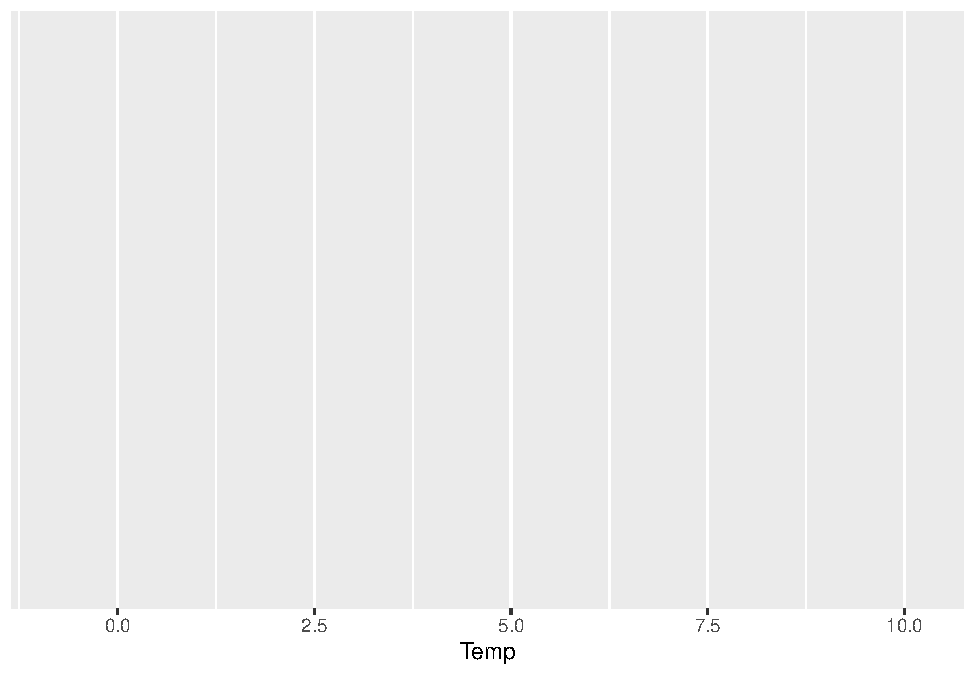
\includegraphics{Chapter-1-Interactive-Notebook-for-Instructors---pp_files/figure-beamer/unnamed-chunk-19-1.pdf}
\end{frame}

\begin{frame}[fragile]
Let us code the computation of covariance and correlation between height
and weight.

\begin{Shaded}
\begin{Highlighting}[]
\FunctionTok{cov}\NormalTok{(ghw}\SpecialCharTok{$}\NormalTok{weight,ghw}\SpecialCharTok{$}\NormalTok{height)}
\end{Highlighting}
\end{Shaded}

\begin{verbatim}
## [1] 0.6773
\end{verbatim}

\begin{Shaded}
\begin{Highlighting}[]
\FunctionTok{cor}\NormalTok{(ghw}\SpecialCharTok{$}\NormalTok{weight,ghw}\SpecialCharTok{$}\NormalTok{height)}
\end{Highlighting}
\end{Shaded}

\begin{verbatim}
## [1] 0.4379
\end{verbatim}
\end{frame}

\begin{frame}{Some Useful Resources}
\protect\hypertarget{some-useful-resources}{}
\begin{enumerate}
\tightlist
\item
  The R reference card is very useful if you want to look up the basic
  syntax. You are strongly recommended to download and keep it handy as
  you work to get comfortable with coding in R.
  \href{https://cran.r-project.org/doc/contrib/Short-refcard.pdf}{R
  Reference Card}
\item
  There are a number of other cheatsheets for specific packages and
  functionalities. You can find a list of them at
  \href{https://rstudio.com/resources/cheatsheets/\%3E}{Cheatsheets}\\
\item
  \href{https://www.statmethods.net/}{Quick-R}
\end{enumerate}
\end{frame}

\end{document}
